\documentclass[10pt]{article}
\usepackage{url}
\usepackage{color,graphicx}
\usepackage{amssymb,amsmath,amsthm,subfigure}
\usepackage[numbers]{natbib}
\usepackage{algorithm2e}
%\usepackage{almostfull}

%%% Environment for notation and a symbol command to go along with it.
%%% The argument should be the widest symbol which is expected if 
%%% \sym will be used to make the list.
%%%
\newenvironment{notation}[1]{%
\begin{list}{}{\small
\settowidth{\labelwidth}{{#1}\quad}%
\setlength{\itemsep}{1.5pt plus 0.5pt minus 0.2pt}%
\setlength{\parsep}{0ex}%
\setlength{\rightmargin}{0em}%
\setlength{\leftmargin}{\labelwidth}%
\addtolength{\leftmargin}{\labelsep}%
\addtolength{\leftmargin}{1em}}}{\end{list}}

\newcommand{\sym}[1]{\item[${#1}$\hfill{}]}

\newcommand{\bx}{\mathbf{x}}
\newcommand{\bu}{\mathbf{u}}
\newcommand{\tx}{\tilde{x}}
\newcommand{\norm}[1]{\vert #1 \vert}
\newcommand{\set}[1]{\left\lbrace #1 \right\rbrace}
%\newcommand{\SetAlgoLined}{}

\newcommand{\I}{\mathcal{I}}
\newcommand{\BO}{\textrm{BO}}
\newcommand{\IP}{\textrm{Ip}}
\newcommand{\UP}{\textrm{Up}}
\newcommand{\DN}{\textrm{Dn}}
\newcommand{\Inv}{\textrm{Iv}}
\newcommand{\Dem}{\textrm{Dm}}
\newcommand{\ulambda}{\underline{\lambda}}
\newcommand{\olambda}{\overline{\lambda}}
\newcommand{\eig}{\text{eig}}
\newcommand{\diag}{\text{diag}}

\newtheorem{assumption}{Assumption}
\newtheorem{theorem}[assumption]{Theorem}
\theoremstyle{definition}
\newtheorem{algo}[assumption]{Algorithm}
\newtheorem{definition}[assumption]{Definition}
\newtheorem{proposition}[assumption]{Proposition}
\newtheorem{remark}[assumption]{Remark}

\title{Cooperative  model predictive control: Current status and  limitations }
\author{Kaushik Subramanian \thanks{Department of Chemical and Biological
     Engineering, University of Wisconsin-Madison, U.S.A.}  \and James
  B. Rawlings\footnotemark[1] \thanks{Corresponding author: rawlings@engr.wisc.edu}}  
\begin{document}
\maketitle
\begin{abstract}
In this paper, we summarize the current status of cooperative model
predictive controllers for linear systems. We outline the suboptimal
MPC theory that is used to guarantee closed loop properties of
cooperative MPC and describe two methods to relax the centralized control problem to ensure that cooperative MPC
iterates converge to the Pareto optimal solution of the relaxed optimization problem. Finally, we introduce a robust cooperative MPC algorithm based on tube-based MPC
\end{abstract}

\section{Introduction}
\label{sec:introduction}
 Over the
past two decades, model predictive control (MPC) has emerged as one of the
most commonly used control strategies in the process industry. MPC is
an optimization based control algorithm in which a model of the
process is used to predict the future evolution of the process under
different inputs. The best among these input sequences are selected by
solving an optimization problem that also includes the constraints of
the system. However, only the first of these optimal inputs are
injected to the plant, and the whole procedure (along with state
estimation and data reconciliation) is repeated at the next
sampling time, thereby incorporating feedback. MPC is widely used in
many industries like Petrochemicals, fine chemicals, food, automotive
and aerospace etc. \citep{qin:badgwell:2003}

Since only the first input is used and the optimization problem is
solved at the next sampling time, it is important to provide
guarantees that the control objectives are met in the
closed-loop. Stability theory provides the theoretical support and the
guidelines to design the open-loop optimization problem so that the
desirable closed-loop properties (like asymptotic stability to the
set-point) are guaranteed. Stability theory for MPC can either be (i)
Optimal MPC, in which it is required that the online optimization
problem be solved to optimality to ensure closed-loop stability  or (ii) Suboptimal MPC, in which
suboptimal solutions to the online optimization problems that have
certain properties are shown to be enough to ensure closed-loop
stability \citep[Chap 2]{rawlings:mayne:2009}. We discuss Optimal and suboptimal MPC in section \ref{sec:suboptimal}

Chemical plants are composed highly interconnected subsystems that
exchange material, energy and information with one another. As model
predictive controllers are being developed for more and more
processes, the focus is shifting towards plant-wide control. Plant-wide
control strategies must take into account the interactions between the
many different subsystems that comprise the plant. 

Centralized MPC is one way of achieving plant-wide control. In centralized model predictive control, the whole plant is considered
as a single system and a monolithic controller is designed. Although
offering good performance, the centralized controller can be hard to
implement and maintain. 

At the other end, in decentralized control, the plant is
decomposed into many weakly interacting subsystems and the subsystems
are controlled independently \citep{sandell:varaiya:athans:safonov:1978}. It has been shown that decentralized
control can make the plant unstable \citep{cui:jacobsen:2002}. It has
also been shown that the so-called Noncooperative MPC, in which the
subsystems share objective functions but not constraints can also
destabilize the plant \citep{venkat:2006}.

The middle ground is distributed
control, in which we seek to coordinate multiple controllers
\citep{scattolini:2009}. A lot of research focus has been dedicated to
distributed control strategies over the past decade. The preferred architecture for distributed MPC is a
parallel optimization problem to solve the centralized control
problem. In this architecture, each subsystem solves a part of the
centralized control optimization problem. Based on the parallel
optimization algorithm used, we can classify distributed MPC into
three broad categories. Parallel optimization
algorithms based on the dual of the centralized optimization problem
form a class of distributed MPC algorithms. These algorithms use
centralized MPC stability theory for ensuring closed-loop
properties. However, they require that the subsystems converge to the
optimal solution (with the intermediate iterates generally being
infeasible). These algorithms may also require a coordinator.  The second family of distributed MPC algorithms are the
so-called negotiation based methods. In these algorithms, the
subsystems find a feasible, but suboptimal input based on
negotiations. The stability results for this family of algorithms is
based on suboptimal MPC theory. The main drawback of these methods is
that they do not provide any convergence properties. A brief survey of
results belonging to both these classes of distributed MPC algorithms
is provided in Section \ref{sec:related}. In this paper, we review
cooperative MPC. In cooperative MPC, we use the Gauss-Jacobi parallel
optimization algorithm. We modify the centralized MPC
optimization problem so that (i) every iterate is feasible and ensures
cost-drop for the centralized optimization problem and (ii) the
iterations converge to the centralized optimal solution. Therefore,
this family of distributed MPC algorithms (i) requires no coordinator/
coordinating layer, (ii) ensure stability using suboptimal MPC theory
and, (iii) ensure convergence to optimal solution on convergence. 

In this paper, (i) we summarize the methods for cooperative MPC for linear
systems and discuss the advantages and disadvantages of each method
and (ii) propose a robust cooperative MPC algorithm based on
tube-based robust MPC \citep[Chapter 3]{rawlings:mayne:2009}.


In Section \ref{sec:suboptimal}, we briefly overview suboptimal MPC
theory which is the base upon which cooperative MPC is built. In Section \ref{sec:coop} we present the cooperative MPC algorithm and two modifications to the centralized control problem to ensure performance guarantees,  namely,(i) Using Kalman decomposition of the state space (\ref{sec:substate})
and (ii) Using a relaxation of the terminal region
(\ref{sec:relaxation}). In Section \ref{sec:tube}, we present the
tube-based cooperative MPC algorithm for robust cooperative
control. Finally, in Section \ref{sec:related}, we briefly outline
related work in cooperative MPC before concluding in Section
\ref{sec:conclusions}.

\section{MPC Stability theory}
\label{sec:suboptimal}
As mentioned in the previous section, to study the model predictive controller, we need to focus, not only on the
optimization problem solved at each sampling time, but also on the
dynamics of the system with the injected move. Lyapunov theory is an
convenient tool to study the stability and convergence properties of
dynamic systems and MPC design procedures using Lyapunov theory has
been widely studied. In Optimal MPC \citep[Chapter
  2]{rawlings:mayne:2009}, the on-line optimization problem needs to
be solved to optimality to ensure closed-loop properties like
stability and asymptotic convergence. In Suboptimal MPC
\citep{pannocchia:rawlings:wright:2011,scokaert:mayne:rawlings:1999},
the same closed-loop properties can be ensured without requiring
the on-line problems to be solved to optimality. In this section, we briefly review the design procedure for ensuring
closed-loop stability in suboptimal MPC.
 
\subsection{Preliminaries}
Consider a system comprising of $M$ subsystems described by the
following linear dynamics: 
\begin{gather}
\label{eq:mpc:distributed:dynamics}
x_i^+ = A_i x_i + B_{ii} u_i + \sum_{l \in \set{1,2,\ldots,M} \atop l \neq i}
B_{il} u_l \\
x_i \in \mathbb{X}_i \qquad u_i \in
\mathbb{U}_i \label{eq:mpc:distributed:constraints} 
\end{gather}
in which $x_i,u_i$ are the states and inputs in subsystem $i$.

Denoting $x = (x_1,x_2,\ldots,x_M)$ and $u = (u_1,u_2,\ldots,u_M)$, the model can be written as
\begin{equation}
\label{eq:model}
x^+ = Ax + Bu
\end{equation}
The states of the system are described by $x$, while $x^+$ denotes the
state at the next sampling instance.  The states are constrained to lie in the set $\mathbb{X}$ while the inputs are constrained to lie in the set $\mathbb{U}$.

The MPC objective function is defined as:
\begin{equation}
\label{eq:VN0}
V_N(x,\bu) = \sum_{j=0}^{N-1}\ell(x(j),u(j)) + V_f(x(N))
\end{equation}
in which $N$ is the control horizon, $\bu = (u(0),u(1),\ldots,u(N-1))$
is the input vector and $x(j)$ is the short-hand notation for the
state evolution under the input $\bu$. That is,
 \[x(j) = \phi(j;x,\bu)=  A^{j-1}x +\sum_{l=0}^{j-1} A^lBu(j-1-l)\]

The cost function $V_N(x,\bu)$ consists of the stage cost
$\ell(x(j),u(j))$ and the terminal cost $V_f(x(N))$. The costs are
chosen to be positive definite quadratic cost:
\begin{equation}
\label{eq:costs}
\ell(x,u) = \sum_i1/2 (x_i'Q_ix_i + u_i'R_iu_i) \qquad V_f(x) = 1/2x'Px 
\end{equation}
in which $R_i>0, Q_i>0,P > 0$. Note that the the terminal cost $V_f(x)$ is not written as a sum of the terminal costs of the $M$ subsystems. For simplicity, we refer to the matrix $\text{diag}(Q_1,Q_2,\ldots,Q_M)$ as $Q$. Similarly $\text{diag}(R_1,R_2,\ldots,R_M)$ is referred to as $R$.

The on-line optimization problem that is solved is:

\begin{xalignat}{2}
\mathbb{P}_N(x): & \min_{\bu}V_N(x,\bu) & \nonumber \\
& \text{s.t~} x(j+1) = Ax(j) + Bu(j)&  \forall j \in 0,1,\ldots,N-1\nonumber\\
& x(j) \in \mathbb{X},&   \forall j \in 0,1,\ldots,N-1 \nonumber \\
& u(j) \in \mathbb{U}, &\forall j \in 0,1,\ldots,N-1  \label{eq:PNx}\\
& x(0) = x \nonumber \\
& x(N) \in \mathbb{X}_f \nonumber
\end{xalignat}
The set $\mathbb{X}_f$ is called as the terminal region.

We define the set $\mathbb{Z}$ as the feasible region of the problem
$\mathbb{P}_N(x)$. That is,

\begin{equation}
\label{eq:Zopt}
\mathbb{Z} = \set{(x,\bu) \mid \phi(j;x,\bu) \in \mathbb{X},
  \phi(N;x,\bu) \in \mathbb{X}_f, \bu \in \mathbb{U}^N}
\end{equation}

The projection of the feasible space onto $x$ is the set of feasible
inputs for a given initial state $x$. This set is denoted by
$\mathcal{U}_N(x)$ and is given by:

\[ \mathcal{U}_N(x) = \set{\mathbb{\bu} \mid (x,\bu) \in \mathbb{Z}}
\]

The following assumptions are made on the system:
\begin{assumption}
\label{ass:stab}
The centralized system $(A,B)$
is stabilizable.  
\end{assumption}

\begin{assumption}
\label{ass:psd}
The cost functions $\ell(x,u)$ and $V_f(x)$ are positive definite.
\end{assumption}
\begin{assumption}
\label{ass:bsa}
The set $\mathbb{X}_f$ and the  costs $\ell(x,u),V_f(x)$ are chosen
such that there exists a controller $u = \kappa_f(x)$ that satisfies:
\begin{xalignat}{1}
\label{eq:bsa}
V_f(Ax+B\kappa_f(x)) -V_f(x) \leq -\ell(x,\kappa_f(x)) &\qquad \forall x
\in \mathbb{X}_f \\
Ax + B\kappa_f(x) \in \mathbb{X}_f, \kappa_f(x) \in \mathbb{U}& \qquad
\forall x \in \mathbb{X}_f
\end{xalignat}
\end{assumption} 

\begin{assumption}
\label{ass:closed}
The set $\mathbb{U}$ is convex, closed and compact and contains the origin in
its interior. The set $\mathbb{X}$ is convex, closed and contains the origin
in its interior. The set $\mathbb{X}_f$ is convex, closed and compact and
contains the origin in its interior.
\end{assumption}

\begin{remark}
Assumption \ref{ass:stab} ensures that a feedback linear controller $u = Kx$ and a cost function $V_f(x) = 1/2 x'Px$ exist such that $P>0$ and the closed-loop $x^+ = (A+BK)x$ is stable. For any $K$ such that $(A+BK)$ is stable, we can find the terminal penalty by solving the Lyapunov equation (the existence of a solution to the Lyapunov equation is guaranteed by Assumption \ref{ass:psd}):
\[ (A+BK)'P(A+BK) + (Q+K'RK) = P \]

The control invariant region in which the feedback controller $u=Kx$ is feasible is then the set $\mathbb{X}_f$ defined as:
\[ \mathbb{X}_f := \set{x \mid x^+= (A+BK)x \in \mathbb{X}_f \subseteq
  \mathbb{X}, Kx \in \mathbb{U}}
\]

See \citet{gilbert:tan:1991} for an algorithm to construct such sets for linear systems.
\end{remark}

\begin{remark}
Assumption \ref{ass:bsa} also ensures that the following identity is true for any $\beta \geq 1$
\[\beta V_f(Ax+B\kappa_f(x)) + \ell(x,\kappa_f(x)) \leq \beta
V_f(x) \]
\end{remark}
\subsection{Optimal MPC}
The optimal solution to the optimization problem \eqref{eq:PNx} is
denoted by $\bu^0(x)$ and the optimal objective value is given by
$V_N^0(x)$. We define the optimal MPC law as $\kappa_0(x) = u^0(0;x)$
in which $u^0(0;x)$ is the first input in the optimal sequence
$\bu^0(x)$. The close-loop is hence $x^+ = Ax + B\kappa_0(x)$. The
centralized MPC asymptotic (exponential) stabiity theorem \citep[Thm 2.24(b),
  Chap. 2]{rawlings:mayne:2009} is given by Theorem \ref{thm:mpc:optimal}.
\begin{theorem}[Optimal MPC stabilty]
\label{thm:mpc:optimal}
Let Assumptions \ref{ass:stab}--\ref{ass:closed} hold. Then
the origin is exponentially stable with a region of attraction
$\mathcal{X}_N$ for the system $x^+ = Ax + B\kappa_0(x)$. If
$\mathcal{X}_N$ is unbounded, then the region of attraction is any
sublevel set of $V_N^0(\cdot)$.
\end{theorem}

The detailed  proof for Theorem \ref{thm:mpc:optimal} is
provided in \citet[Chap. 2]{rawlings:mayne:2009}.

\subsection{Suboptimal MPC}
As the name suggests, in suboptimal MPC, we wish to inject {\emph{some}} feasible input
to the plant. There could be several reasons to inject suboptimal
input sequences. For example, the sampling time might be too small to
solve the problem to optimality.  In order to ensure that despite injecting suboptimal
inputs to the plant, we maintain the desirable closed-loop properties,
we define the warm start and the successor input set as follows. We
denote $\kappa_s(x)$ as the first input in the suboptimal input
sequence.

\begin{definition}[Warm Start]
\label{def:warmstart}
Let $(x,\bu)$ be a state-input vector pair such that $\bu \in \mathcal{U}_N(x)$ (that is $\bu$ is feasible
for $\mathbb{P}_N(x)$).  Then the warm start for the successor initial state
$x^+ = Ax+B\kappa_s(x)$ is defined as:
\begin{equation*}
%\label{eq:warmstart}
\tilde{\bu} = \left (\bu(1;x),\bu(2;x),\ldots,\bu(N;x),u_+\right)
\end{equation*}
in which  $u_+ = \kappa_f(\phi(N;x,\bu))$.
\end{definition}
\begin{definition}[Successor input set]
\label{def:G}
Consider $(x,\bu)$ such that $\bu$ is feasible for
$\mathbb{P}_N(x)$. For the  successor state 
$x^+ = Ax+B\kappa_s(x)$, we define the set $G(x,\bu)$
\begin{multline*}
G(x,\bu) = \lbrace \bu^+ \mid \bu^+ \in
\mathcal{U}_N(x^+), V(x^+,\bu^+)\leq V(x,\tilde{\bu}), \\
V(x^+,\bu^+) \leq V_f(x^+) \text{~if~} x\in r\mathbb{B} \rbrace
\end{multline*}
in which $\tilde{\bu}$ is the warm start given by Definition 
\ref{def:warmstart} and $r\mathbb{B}$ is a ball of radius $r>0$. We
choose $r$ sufficiently small such that  
$r\mathbb{B}$ is a subset of the terminal region.
\end{definition}
Additionally, we make the 
following assumptions on the cost function $V_N(x,\bu)$.

\begin{assumption}
\label{ass:mpc:suboptimalconstants}
There exist positive constants $a,a_1',a_2',a_f$ and $r$, such
that the cost function $V_N(x,\bu)$ satisfies:
\begin{alignat*}{2}
\ell(x,u) &\geq a_1' \norm{(x,u)}^a &\qquad (x,u) &\in \mathbb{X} \times \mathbb{U} \\
V_N(x,\bu) &\leq a_2' \norm{(x,\bu)}^a &\qquad (x,u) &\in
\mathcal{B}_{r} \\
V_f(x) &\leq a_f\norm{x}^a &\qquad x &\in \mathbb{X}
\end{alignat*}
in which $\mathcal{B}_{r}$ is the ball of radius $r$.
\end{assumption}

Note that it is easy to show that Assumption
\ref{ass:mpc:suboptimalconstants} is satisfied for linear systems and
quadratic costs.

The suboptimal MPC optimization problem can
be  written as:
\begin{xalignat}{2}
\mathbb{P}_N(x): & \min_{\bu}V_N(x,\bu) & \nonumber \\
& \text{s.t~} x(j+1) = Ax(j) + Bu(j)&  \forall j \in 0,1,\ldots,N-1\nonumber\\
& x(j) \in \mathbb{X},&   \forall j \in 0,1,\ldots,N-1 \nonumber \\
& u(j) \in \mathbb{U}, &\forall j \in 0,1,\ldots,N-1  \label{eq:PNx_Sub}\\
& x(0) = x \nonumber \\
& x(N) \in \mathbb{X}_f \nonumber \\
& \norm{\bu} _i\leq d_i \norm{x}, &\forall i \in 1,2,\ldots,M,\nonumber\\
& & \forall x \in \mathcal{B}_r \nonumber
\end{xalignat}

\begin{theorem}
\label{thm:suboptimal}
Let Assumptions \ref{ass:stab} --\ref{ass:closed} and \ref{ass:mpc:suboptimalconstants}
hold. Choose optimization problem $\mathbb{P}_N(x)$ given by \eqref{eq:PNx_Sub} and the appropriate terminal
regions. For any $x$ for which  $\mathcal{U}_N(x)$  is not empty, choose
$\bu \in \mathcal{U}_N(x)$. Then, the origin of the closed-loop system 
\begin{align*}
x^+ &= Ax+ B\kappa_s(x) \\
\bu^+ &\in G(x,\bu)
\end{align*}
is asymptotically stable on (arbitrarily large) compact  subsets of
the feasible region $\mathcal{X}_N :=\set{x\mid \exists u \in
  \mathbf{U}^N, \text{~s.t~} \mathcal{U}_N(x) \neq \varnothing}$. 
\end{theorem}

The proof of Theorem \ref{thm:suboptimal} is presented in
\citep{pannocchia:rawlings:wright:2011}.

Observe that for the nominal system, the warm start is a member of the
set $G(x,\bu)$ because of Assumption \ref{ass:bsa}.  Therefore, if we have a feasible $(x,\bu)$ pair, we
can construct an asymptotically stable closed loop without any
optimization. In-fact, if the optimization algorithm used to solve the
on-line MPC problem generates feasible iterates which decrease the
objective value, then we can stop the optimizations at any suboptimal
solution and inject that solution to the plant and ensure asymptotic
stability. Further, note that unlike the optimal MPC optimization
problem, the on-line problem for suboptimal MPC has an extra
constraint, namely, $V(x^+,\bu^+) \leq V_f(x^+) \forall x \in
\mathcal{B}_r$. This constraint can also be written
as $\norm{\bu} \leq d \norm{x}, d>0, \forall x \in
\mathcal{B}_r$.  We can show that
this constraint is equivalent to  $\norm{\bu_i} \leq d_i \norm{x}, x \in
r\mathbb{B},d_i >0, i \in 1,2,\ldots,M$
\citep{subramanian:rawlings:maravelias:2012} in which $\bu_i =
(u_i(0), u_i(1), \ldots, u_i(N-1))$ and $i$ denotes the input of
subsystem $i$. 

For future reference, we define the following set:
\begin{equation}
\label{eq:mpc:UN_sub}
\mathcal{U}_N^{s}(x;r) := \set {u \mid u \in \mathcal{U}_N(x),\norm{\bu} \leq d \norm{x}  \text{ if~} x \in
\mathcal{B}_r}
\end{equation}

In the following section, we discuss the design of the on-line
optimization problem for cooperative MPC algorithm that establishes
stability using suboptimal MPC theory.

\section{Cooperative MPC}
\label{sec:coop}
In Cooperative MPC, we assume that each subsystem knows (i) the
overall system model \eqref{eq:model} and (ii) the overall system
objective function \eqref{eq:VN0}. With the knowledge of the system-wide model and objective
function, each subsystem then solves the centralized
MPC problem \eqref{eq:PNx_Sub}. Each subsystem shares (i) its current
decision variable $\bu_i$ with all the other subsystems, (ii)
optimizes the centralized problem over its decision variables having
fixed the decision variables of the other sub-systems at the shared
value, and (iii) makes the control move without requiring any
coordinating layer. The cooperative MPC algorithm is presented in Algorithm \ref{alg:coop}.

For subsystem $i$, we denote all the other subsystems as
$-i$. The following is the optimization problem for subsystem
$i$ . The input of all other subsystems is denoted by $\bu_{-i}$. That is,
\[\bu_{-i} =
(\bu_1,\bu_2,\ldots,\bu_{i-1},\bu_{i+1},\ldots,\bu_M)\]

\begin{xalignat}{2}
\mathbb{P}^{i}_N(x,\mathbf{v}_{-i}): & \min_{\bu_i}V_N(x,\bu)& \nonumber \\
& \text{s.t~} x(j+1) = Ax(j) + Bu(j) & \forall j \in 0,1,\ldots,N-1\nonumber\\
& x(j) \in \mathbb{X}&\forall j \in 0,1,\ldots,N-1\nonumber \nonumber \\
& u(j) \in \mathbb{U}&\forall j \in 0,1,\ldots,N-1\nonumber \nonumber \\ 
& u_{-i}(j) = v_{-i}(j),  \qquad & \forall j \in 0,1,\ldots,N-1 \nonumber \\
& x(0) = x& \label{eq:PNxu} \\
& x(N) \in \mathbb{X}_f& \nonumber \\
& \norm{\bu_i} \leq d_i \norm{x} & \forall{x} \in \mathcal{B}_r \nonumber
\end{xalignat}

\begin{algo}[Cooperative MPC] \mbox{}
\label{alg:coop}
\begin{algorithm}
 \KwData{Starting state $x(0)$, initial guess
   $(\tilde{\bu}_1(0),\tilde{\bu}_2(0),\ldots,\tilde{\bu}_M(0)) \in \mathcal{U}^s_N(x(0);r)$,
   $\bar{p} \geq 1$ and $\omega_i \in (0,1)$ such that
   $\sum_{i=0}^{M}\omega_i = 1$}
 \KwResult{Closed loop $(x(j),u(j)), j = \set{1,2,\ldots}$}
 set $j \leftarrow 0$ \\
 \While {$j \geq 0$}{
   Set $p \leftarrow 0$, $x \leftarrow x(j)$\\
   Set $\bu_i^{(p)} \leftarrow \tilde{\bu}_i(j)$ for $i = 1,2,\ldots,M$\\
   Broadcast current subsystem inputs $\tilde{\bu}_i(j)$ to other
   subsystems \\
   \While {$p < \bar{p}$}{
       Solve $\min_{\bu_i}{V_N(x,\bu)} \quad \text{s.t.~} \bu \in
       \mathcal{U}_N^s(x;r); \bu_{-i} = \bu_{-i}^{(p)}$ to obtain
       $\bu_i^0$ for i in $1,2,\ldots,M$ \\
       Set $\bu_i^{(p+1)} \leftarrow \omega_i \bu_i^{(p)} +
       (1-\omega_i) \bu_i^0$ for i in $1,2,\ldots,M$ \\
       Set $p \leftarrow p+1$\\
   }
  Set $\bu \leftarrow (\bu_1^{(p)},\bu_2^{(p)},\ldots,\bu_M^{(p)})$ and find $x(j+N) \leftarrow
  \phi(N;x(j),\bu)$\\
  Obtain $u_+ = (u_{1+},u_{2+},\ldots,u_{M+}) \leftarrow \kappa_f(x(j+N))$\\
  Obtain warm start $\tilde{\bu}_i(j+1) =
    (\bu_i^{(p)}(1),\bu_i^{(p)}(2),\ldots,u_{i+})$ for $i = 1,2,\ldots,M$.\\
   Set input as $u(j) =
  (\bu_1^{(p)}(0),\bu_2^{(p)}(0),\ldots,\bu_M^{(p)}(0))$\\
  Evolve state from $x(j)$ to $x(j+1)$ under input $u(j)$\\
  Set $j \leftarrow j+1$ \\
 }
\end{algorithm}
\end{algo}

In the inner loop in Algorithm \ref{alg:coop}, all the subsystems are
solving the same optimization problem, but with the inputs of the
other subsystem fixed. Each system, having solved the optimization
problem, takes the convex combination of its optimal solution and the
starting point. This algorithm is the implementation of the Jacobi
parallel optimization routine \citep[Section 3.3.5]{bertsekas:tsitsiklis:1989}. For convex optimization problem
(convex objective and convex constraints), the Jacobi optimization
generates feasible iterates that decrease the objective function value
(when initialized from a feasible starting iterate). Hence, from the
conclusions of the previous section, we can use suboptimal MPC theory
to ensure stability of the cooperative MPC algorithm. 

Before presenting the cooperative MPC stability theorem
(which in different forms have been stated in
\citet{stewart:venkat:rawlings:wright:pannocchia:2010, venkat:2006, stewart:wright:rawlings:2011, subramanian:rawlings:maravelias:2012}), we
briefly review the properties of Jacobi algorithm for convex
optimization problem.

\subsubsection*{Jacobi algorithm}
For the sake of simplicity, we consider only two subsystems in this
section. Consider the following optimization problem
\eqref{eq:mpc:distributed:coop:jordan}, solved using 
Algorithm \ref{alg:mpc:distributed:coop:jordan}.

\begin{equation}
\label{eq:mpc:distributed:coop:jordan}
\mathbb{J} : \min_{y_1,y_2}{J(y_1,y_2)} \qquad \text{s.t.~} (y_1,y_2)\in \Omega 
\end{equation}
in which $J(\cdot)$ is a convex function and $\Omega$ is a convex,
closed and compact set. 

\begin{algo}[Jacobi algorithm \citep{bertsekas:tsitsiklis:1989}] \mbox{ }

\label{alg:mpc:distributed:coop:jordan}
\begin{algorithm}[H]
 \KwData{Starting guess $(y_1,y_2) \in \Omega$
    and $\omega_i \in (0,1)$ such that
   $\sum_{i=1}^{2}\omega_i = 1$}
 \KwResult{Sequence of feasible iterates $\set{y^{(p)}}$ and
   non-increasing objective function values $\set{J(y^{(p)})}$}
 Set $p \leftarrow 0$\\
  \While {$p \geq 0$}{
   Set  $y_1^{(p)} \leftarrow y_1$, $y_2^{(p)}
   \leftarrow y_2$\\
   Solve $\min_{y_1}{J(y_1,y_2)}, \text{s.t.~} y_2 = y_2^{(p)},
   (y_1,y_2) \in \Omega$  to obtain $y_1^0$. \\
   Solve $\min_{y_2}{J(y_1,y_2)}, \text{s.t.~} y_1 = y_1^{(p)},
   (y_1,y_2) \in \Omega$  to obtain $y_2^0$. \\
   Set $y_i^{(p+1)} \leftarrow \omega_i y_i^{(p)} +
       (1-\omega_i) y_i^0$  for i in $1,2$ \\
       Set $p \leftarrow p+1$\\
   }
\end{algorithm}
\end{algo}

Proposition \ref{prop:mpc:distributed:jordan} establishes that all iterates generated by the Jacobi algorithm for a convex optimization problem are feasible and decrease the objective function value.
\begin{proposition}
\label{prop:mpc:distributed:jordan}
Let $J(y)$ be continuously differentiable and strongly
convex function on the convex, closed and  compact set $\Omega$.
Let Algorithm \ref{alg:mpc:distributed:coop:jordan} be used to solve
convex optimization problem \eqref{eq:mpc:distributed:coop:jordan}
from an initial feasible point $y \in \Omega$. Then, (i) every iterate
$y^{(p)}$ generated by the algorithm is feasible and , (ii)
$J(y^{(p+1)}) \leq J(y^{(p)}), \forall p>0$.
\end{proposition}
The proof is provided in  \citet{stewart:venkat:rawlings:wright:pannocchia:2010}.

Proposition \ref{prop:mpc:distributed:jordan} does not establish any property about the convergence of the iterates generated by the Jacobi algorithm. In order to establish that the iterates converge to the optimal solution of the problem \eqref{eq:mpc:distributed:coop:jordan}, we require a much stricter condition on the constraints. Proposition \ref{prop:mpc:distributed:jordan:converge} lists the requirements on the optimization problem to ensure that the iterates generated by the Jacobi algorithm converge to the optimal solution.
\begin{proposition}
\label{prop:mpc:distributed:jordan:converge}
Let $J(y)$ be continuously differentiable and strongly
convex. Let $\Omega = \Omega_1 \times \Omega_2$, in which $y_1 \in
\Omega_1$ and $y_2 \in \Omega_2$, with $\Omega_i$  convex, closed and compact. Then, as $p
\rightarrow \infty$, the iterates $y^{(p)}$ converges to the $y^o$, in
which $y^o$ is the optimal solution to optimization problem
\eqref{eq:mpc:distributed:coop:jordan}
\end{proposition}  
This proof is provided in  \citet{stewart:venkat:rawlings:wright:pannocchia:2010}. Another
proof is also provided in \citet[Prop 3.9]{bertsekas:tsitsiklis:1989}
for Gauss-Seidel algorithm which is closely related to the Jacobi
algorithm.  Note that the important requirement in \ref{prop:mpc:distributed:jordan:converge} is that the constraints be uncoupled.

We now present the exponential stability of the cooperative MPC algorithm.
\begin{theorem}
Let Assumptions \ref{ass:stab} -- \ref{ass:closed} and
\ref{ass:mpc:suboptimalconstants} 
hold. Choose $r>0$ such that $\mathcal{B}_r \subset \mathbb{X}_f$. For
any $x$ for which  $\mathcal{U}_N^s(x;r)$  is not empty, choose 
$\bu \in \mathcal{U}_N^s(x;r)$. Then, the origin of the closed-loop system 
obtained by Algorithm \ref{alg:coop}
is exponentially stable. The region of attraction are (arbitrarily large) compact  subsets of
the feasible region \[\mathcal{X}_N :=\set{x\mid \exists u \in
 \mathbf{U}^N, \text{~s.t~} \mathcal{U}^s_N(x;r) \neq \varnothing}\]
\end{theorem}
We present a sketch of the proof below. The detailed proof is
availalbe in  \citet{stewart:venkat:rawlings:wright:pannocchia:2010}.

We show that the closed-loop system obtained by Algorithm
\ref{alg:coop} is an implementation of suboptimal MPC
and use Theorem \ref{thm:suboptimal} to prove exponential
stability. The optimization problem solved by the Jacobi algorithm in
cooperative MPC is the centralized suboptimal MPC optimization problem \eqref{eq:PNx_Sub}
We note that the optimization problem \eqref{eq:PNx_Sub} 
has convex constraints and a strongly convex objective. By choice
$Q,R,P>0$, we know that the objective function is positive definite
and hence strongly  convex. Using Assumption \ref{ass:closed}, we
can conclude that the constraints are convex, that is
$\mathcal{U}_N(x)$ is convex. 
The set
$\mathcal{U}_N^{s}(x;r)$ is the intersection of two convex
sets, namely, the convex set $\mathcal{U}_N(x)$ and the level set
$V_f(x,\bu) \leq V_f(x) \forall x \in \mathcal{B}_r$. Therefore
$\mathcal{U}_N^s(x;r)$ is convex as well. Hence, by Proposition \ref{prop:mpc:distributed:jordan}, we know
that  if $(x,\tilde{\bu})$ is feasible for
\eqref{eq:PNx_Sub} then (i) {\emph{all}} the iterates generated by the inner loop in  Algorithm
\ref{alg:coop} are feasible; implying $\bu^{(p)} \in
\mathcal{U}_N^{s}(x;r)$ and, (ii) the cost at iterate $p$ is not
greater than the cost achieved by $V_N(x,\tilde{\bu})$; that is
$V_N(x,\bu^{(p)}) \leq V_N(x,\tilde{\bu})$. 

By choice of $\tilde{\bu}(0)$, we know that $(x(0),\tilde{\bu}(0))$ is
feasible for \eqref{eq:PNx_Sub}. Therefore,
$(x(0),\bu^{(p)}(0)) \in \mathbb{Z}_N$ with $V_N(x(0),\bu^{(p)}(0))
\leq V_N(x(0), \tilde{\bu}(0))$. Since $\tilde{\bu}(1)$ is the warm
start constructed from $\bu^{(p)}(0)$, we know that it is feasible and
that $\tilde{\bu}(1) \in G(x(0),\bu^{(p)}(0))$. Therefore, by induction
the closed-loop obtained by
Algorithm \ref{alg:coop} belongs to the family of
closed-loop solutions for which we showed exponential stability in
Theorem \ref{thm:suboptimal}.


\subsection{Performance guarantees}
In showing exponential stability of cooperative MPC algorithm for
linear systems, we used Proposition \ref{prop:mpc:distributed:jordan}
to ensure that all the iterates generated by the cooperative MPC
algorithm are feasible and provide cost-drop. Also, in establishing
the stability of cooperative MPC, we did not modify the on-line
optimization problem solved by the distributed controller. The
distributed controller solves the centralized suboptimal MPC
optimization problem. But, since the centralized suboptimal MPC
optimization problem has coupled constraints (namely, the state
constraints, the input constraint and the terminal constraint. The equality constraints can be eliminated fairly easily); the Jordan parallel optimization
algorithm need not necessarily converge to the optimal
solution. In order to establish performance guarantees (if we let the
cooperative MPC algorithm to converge), we modify the on-line
optimization problem to be solved such that it has no coupled
constraints. By doing so, we ensure that the Jacobi algorithm
converges to the optimal solution of the (re) designed on-line
optimization problem. To ``uncouple'' the constraints, we make further
assumptions on the system as listed below:

\begin{assumption}
\label{ass:noX}
There are no state constraints. State constraints are enforced as
soft-penalties by tuning the $Q$ matrix in the stage cost.
\end{assumption}

\begin{assumption}
\label{ass:uncoupledU}
The input constraint space is uncoupled. That is, the input constraint
set $\mathbb{U}$ is the Cartesian product of the input constraint sets
of each subsystem. 
\[ \mathbb{U} = \mathbb{U}_1 \times \mathbb{U}_2 \times \ldots \times
\mathbb{U}_M
\]
\end{assumption}

Under Assumption \ref{ass:noX} and \ref{ass:uncoupledU}, the only
coupled constraint is the terminal region
constraint which needs to be enforced to guarantee stability and
asymptotic convergence. In the next two sections, we briefly review
two techniques to ``uncouple'' the terminal region constraint.

\subsubsection{Sub-states}
\label{sec:substate}
This relaxation was proposed by \citet{stewart:venkat:rawlings:wright:pannocchia:2010} to solve the terminal equality constraint problem, that is,  $\mathbb{X}_f = \set{0}$.  To uncouple the terminal constraint $x(N) = 0$, we consider the ``sub-state" $x_{il}$. The sub state $x_{il}$ is the part of the state $x_i$ in subsystem $i$ that is {\emph{only}} influenced by input $u_l$ in subsystem $l$.  The sub-state model is a non-minimal realization of the system \eqref{eq:mpc:distributed:dynamics}.  The dynamics for sub-state $x_{il}$ is given by:

\begin{equation}
\label{eq:substate}
 \tilde{x}_{il}^+  = \tilde{A}_{il} x_{il}  + \tilde{B}_{il} u_l
\end{equation}

Defining $\hat{x}_i = \begin{bmatrix} \set{\tilde{x}_{il}}, l =
  {1,2,\ldots,M}\end{bmatrix}$, each subsystem model is given by
  \eqref{eq:mpc:distributed:dynamics}. The matrices
  $\hat{A}_i,\hat{B}_{il}$ are used to describe the dynamics in
  subsystem $i$.
\begin{gather}
\underbrace{\begin{bmatrix} \tilde{x}_{i1}\\\tilde{x}_{i2} \\\vdots\\\tilde{x}_{iM}\end{bmatrix}^+}_{\hat{x}_i^+} =
 \underbrace{\begin{bmatrix} \tilde{A}_{i1} &  & & \\
  & \tilde{A}_{i2}& & \\
  & & \ddots & \\ & & &\tilde{A}_{iM} \end{bmatrix}
 }_{\hat{A}_i}
 \underbrace{\begin{bmatrix} \tilde{x}_{i1}\\
 \tilde{x}_{i2} \\
 \vdots\\
 \tilde{x}_{iM}
 \end{bmatrix}}_{\hat{x}_i}+
 \underbrace{\begin{bmatrix}\tilde{B}_{i1}\\0\\\vdots\\0\end{bmatrix}}_{\hat{B}_{i1}}u_1
 +
 \underbrace{\begin{bmatrix}0\\\tilde{B}_{i2}\\\vdots\\0\end{bmatrix}}_{\hat{B}_{i2}}u_2
 + \ldots
 \underbrace{\begin{bmatrix}0\\0\\\vdots\\\tilde{B}_{iM}\end{bmatrix}}_{\hat{B}_{iM}}u_M
 \label{eq:mpc:distributed:subsystem}
\\
x_i = \underbrace{\begin{bmatrix} \tilde{C}_{i1} & \tilde{C}_{i2} & \ldots & \tilde{C}_{iM}\end{bmatrix}}_{\hat{C}_i}\underbrace{\begin{bmatrix} \tilde{x}_{i1}\\
\tilde{x}_{i2} \\
\vdots\\
\tilde{x}_{iM} \end{bmatrix}}_{\hat{x}_i}
\end{gather}

We assume that the centralized states $x_i$ can be
constructed from the sub-states $\hat{x}_{i}$ (see Assumption
\ref{ass:mpc:distributed:substate:stab}).

The subsystem stage cost $\ell_i(x_i,u_i) = 1/2(x_i'Q_ix_i + u_iR_iu_i)$
can now be written as 
\[ \ell_i(x_i,u_i) = \ell_i(\hat{x}_i,u_i) = 1/2(\hat{x}_i \hat{C}_i'Q_i\hat{C}_i \hat{x}_i +
u_iR_iu_i)\]

The centralized stage cost is $\ell(x,u) = \sum_{i=1}^{M}
\ell_i(\hat{x}_i,u_i)$. Since, we use a terminal constraint that all
states are zero at the end of the horizon, we do not need a terminal penalty.
 
We define $\underline{x}_l$ as the sub-states that are affected by
input $l$. That is $\underline{x}_l = \begin{bmatrix}\set{\tilde{x}_{il}} i =
  \set{1,2,\ldots,M}\end{bmatrix}$. Correspondingly, we define
$\underline{A}_l,\underline{B}_l$ as follows:

\begin{equation}
\underbrace{\begin{bmatrix}
\tilde{x}_{1l}\\
\tilde{x}_{2l}\\
\vdots\\
\tilde{x}_{Ml}
\end{bmatrix}^+}_{\underline{x}_l^+} =
\underbrace{\begin{bmatrix}
\tilde{A}_{1l} & & & \\
& \tilde{A}_{2l} & &  \\
& & \ddots & \\
& & & \tilde{A}_{Ml}
\end{bmatrix}
}_{\underline{A}_l}
\underbrace{\begin{bmatrix}
\tilde{x}_{1l}\\
\tilde{x}_{2l}\\
\vdots\\
\tilde{x}_{Ml}
\end{bmatrix}}_{\underline{x}_l}
+\underbrace{\begin{bmatrix}
\tilde{B}_{1l}\\
\tilde{B}_{2l}\\
\vdots\\
\tilde{B}_{Ml}
\end{bmatrix}
}_{\underline{B}_l}u_l
\label{eq:mpc:distributed:substate:Aunderline}
\end{equation}


The constraint $x_i(N)=0$ can be equivalently written as $\tilde{x}_{il}= 0, l
\in \set{1,2,\ldots,M}$. Therefore, the centralized MPC problem can be written as:

\begin{xalignat}{2}
\mathbb{P}_N(x): & \min_{\bu}V_N(x,\bu)& \nonumber \\
&\text{s.t.~} \underline{x}_l(j+1) = \underline{A}x_l(j) +
\underline{B}_l(j) u_l(j) &j = \set{0,1,2,\ldots,N-1}, \nonumber \\ &&l =
\set{1,2,\ldots,M} \nonumber \\
&x_i(j) = \hat{C}_i \hat{x}_i(j) &j = \set{1,2,\ldots,N}, \nonumber \\ &&i =
\set{1,2,\ldots,M} \nonumber\\
&u_l(j) \in \mathbb{U} &  j =
\set{0,1,2,\ldots,N-1}, \nonumber \\ &&l = \set{1,2,\ldots,M} \nonumber \\
&x_i(0) = x_i & i = \set{1,2,\ldots,M} \nonumber \\
&\underline{x}_l(N) = 0 & l= \set{1,2,\ldots,M}  \label{eq:mpc:distributed:substate:PNx:uncoupled}
\end{xalignat}


Optimization problem \eqref{eq:mpc:distributed:substate:PNx:uncoupled} does not have any coupled constraints as the $\underline{x}_l$ are the set of sub-states that depend only on one input. An alternate explanation is that the each subsystem input stabilizes all the sub-states that it influences in the inner optimizations of the cooperative MPC algorithm.  Since there are no coupled constraints in the optimization problem, the Jacobi algorithm converges to the centralized solution.

Finally, we require that the non-minimal realization satisfies the following assumption to ensure that  (i) the input $\bu_i$ can be used to
zero all the states that $u_i$ influences (feasibility of \eqref{eq:mpc:distributed:substate:PNx:uncoupled}), (ii) all the sub-states can be
reconstructed from the outputs (so that a state estimator can reconstruct $x_{il}$ from measurements of $x_i$). 
\begin{assumption}[Subsystem stabilizability]\mbox{ }
\label{ass:mpc:distributed:substate:stab}
\begin{itemize}
\item The system $(\underline{A}_i,\underline{B}_i)$ is stabilizable.
\item The system $(\hat{A}_i,\hat{C}_i)$ is detectable.
\end{itemize}
\end{assumption}

\begin{remark}
The decomposition into the substate models
\eqref{eq:mpc:distributed:dynamics} can be obtained from the Kalman decomposition of
the original input/output $y_i,u_i$ model
\citep[p.270]{antsaklis:michel:1997}. The drawback however, is that not all centralized stabilizable models
have a corresponding substate non-minimal realization that satisfies
Assumption \ref{ass:mpc:distributed:substate:stab}. One such example is the system of
integrators (like supply chain models \citep{subramanian:rawlings:maravelias:2012}).
\end{remark}


\subsubsection{Relaxing the terminal region}
\label{sec:relaxation}
This relaxation was proposed by
\citet{rawlings:stewart:wright:mayne:2010}, and has been used for
nonlinear suboptimal/ distributed / economic  MPC in
\citet{stewart:wright:rawlings:2011},
\citet{pannocchia:rawlings:wright:2011},
\citet{amrit:rawlings:angeli:2011} as well as linear MPC in
\citet{subramanian:rawlings:maravelias:2012}.

In this relaxation, we (i) Modify the terminal region $\mathbb{X}_f$ to be the sub level set of the terminal cost given by \eqref{eq:Xfa} and (ii) Modify the objective function by magnifying the terminal cost using a parameter $\beta \geq 1$ as shown in \eqref{eq:VNbeta}
\begin{equation}
\label{eq:Xfa}
\mathbb{X}_f := \set{x \mid V_f(x) \leq a, a > 0}
\end{equation}

\begin{equation}
\label{eq:VNbeta}
V_N^\beta(x,\bu) = \sum_{j=0}^{N-1} \ell(x(i),u(i)) + \beta V_f(x(N))
\end{equation}

Note that we choose the parameter $a>0$ such that the set set $\mathbb{X}_f$ given by \eqref{eq:Xfa} satisfies the Assumption \ref{ass:bsa}.

The online optimization problem that is solved is given by:
\begin{xalignat}{2}
\mathbb{P}_N(x): & \min_{\bu}V_N^\beta(x,\bu) & \nonumber \\
& \text{s.t~} x(j+1) = Ax(j) + Bu(j)&  \forall j \in 0,1,\ldots,N-1\nonumber\\
& u(j) \in \mathbb{U}, &\forall j \in 0,1,\ldots,N-1  \label{eq:PNx_Beta}\\
& x(0) = x \nonumber \\
& \norm{\bu}_i \leq d_i \norm{x}, &\forall i \in 1,2,\ldots,M,\nonumber \\ && \forall x \in \mathcal{B}_r \nonumber
\end{xalignat}

Note that in contrast to the suboptimal MPC online problem \eqref{eq:PNx_Sub}, the optimization problem based on relaxing the terminal region \eqref{eq:PNx_Beta} has a magnified terminal penalty (given by $V_N^\beta(x,\bu)$) but {\emph{no}} terminal constraints. Therefore, the Jacobi parallel optimization algorithm on \eqref{eq:PNx_Beta} will converge to the optimal solution. 

However, to ensure closed-loop properties, we need to ensure that every feasible solution to \eqref{eq:PNx_Sub} satisfies the terminal region constraint, that is \eqref{eq:Xfa}. To do so, we design the feasible set of the problem \eqref{eq:PNx_Beta} by appropriate choice of the parameter $\beta$. Recall that for suboptimal and optimal MPC, the feasible set was the set of $(x,\bu)$ pair for which the optimization problems \eqref{eq:PNx} or \eqref{eq:PNx_Sub} was feasible.  In the case of this relaxation, we define the feasible set as the set of $(x,\bu)$ pairs for which the objective cost $V_N^\beta(x,\bu)$ is less than a parameter $\bar{V}>0$. That is:

\begin{equation}
\label{eq:mpc:distributed:relaxation:ZNbeta}
\mathbb{Z}_N^\beta= \set{ (x,\bu) \mid V_N^\beta(x,\bu) \leq \bar{V}, \bu \in
  \mathbb{U}^N}
\end{equation}


Proposition \ref{prop:betabar} gives guidelines for the choice of the parameter $\beta$ based on the parameters $a>0, \bar{V}>0$ , such that any $(x,\bu)$ that lies in the set $\mathbb{Z}_N^\beta$ automatically satisfies the terminal region constraint $V_f(x(N;x,\bu)\leq a$. 

\begin{proposition}
\label{prop:betabar}
Let the cost function be given by $V_N(x,\bu)$ \eqref{eq:VNbeta}. For  $\bar{V}
\geq a $, define $\bar{\beta} := \bar{V}/a$. Then, for any $\beta \geq
\bar{\beta}$ and $(x,\bu) \in \mathbb{Z}_N^\beta$ given by \eqref{eq:mpc:distributed:relaxation:ZNbeta}, we have
that $\phi(N;x,\bu) \in \mathbb{X}_f$ in which $\mathbb{X}_f$ is given
by \eqref{eq:Xfa}. 
\end{proposition}
The proof is by contradiction and is presented in
\citet{subramanian:rawlings:maravelias:2012}.

Since the problem \eqref{eq:PNx_Beta} has no coupled constraints, we
can ensure that the inner-loop of Algorithm \ref{alg:coop} converges
to the optimal solution of \eqref{eq:PNx_Beta}.
  
\begin{remark}
This relaxation based on magnifying the terminal penalty and designing the feasible set is applicable to any system which is stabilizable. In \citet{pannocchia:rawlings:wright:2011}, it was shown that the feasible set $\mathbb{Z}_N^\beta$  can be made as large as $\mathbb{Z}$( the feasible set for the original online MPC optimization problem \eqref{eq:PNx}) by increasing $\bar{V}$. The drawback however is that the Hessian of the subsequent optimization problem can become ill-conditioned.

An important requirement for the cooperative MPC algorithm is that an initial feasible input sequence $\bu^{(0)}$ be provided to initialize the system.  During implementation, the warm start ensures that there is a feasible input sequence for the subsequent state. However, in the presence of uncertainty (model uncertainty) or additive noise, the warm start may not be feasible for the actual subsequent state. In such cases, we have to find a feasible $\bu \in \mathbb{U}^N$ such that $V_N^\beta(x,\bu) \leq \bar{V}$. This problem has coupled constraints, and to the best of our knowledge, no algorithm exists to find a feasible solution in parallel without requiring a coordinator. In the next section, we present an cooperative MPC algorithm based on robust MPC using tubes to overcome this drawback.
\end{remark}


\subsection{Robust cooperative MPC}
\label{sec:tube}
In this section we build a cooperative MPC algorithm based on tube based MPC \cite{langson:chryssochoos:rakovic:mayne:2004} that can be used even when the warm start becomes infeasible.

We consider the system \eqref{eq:model} subject to bounded additive
disturbance as follows:
\begin{equation}
\label{eq:model_dist}
x^+ = Ax +  B u + w
\end{equation}
We make the following assumption on the disturbance:
\begin{assumption}[Bounded disturbance]
\label{ass:W}
The additive disturbance $w$ lies in a compact set $\mathbb{W}$
containing the origin in its interior.
\end{assumption}

The dynamics without the additive disturbance is called the nominal system. The state of the nominal system is denoted by $z$ and input by $v$. That is the nominal system dynamics is given by:
\begin{equation}
\label{eq:model_nominal}
z^+ = Az + B v
\end{equation}

Denoting error $e = x-z$, we can write the error dynamics as (for the same input signal $u$). 
\begin{equation}
\label{eq:error_dynamics}
e^+ = Ax+Bu+w - Az+Bu = Ae + w
\end{equation}

Therefore, given the same initial condition and input sequence, the error at time $k$, $e(k)$ can be shown to lie in the following set:
\begin{equation}
\label{eq:error_set}
e(k) \in S(i) :=\sum_{j=0}^{k-1}A^j\mathbb{W} = \mathbb{W} \oplus A\mathbb{W}
\oplus \ldots \oplus A^{k-1}\mathbb{W}
\end{equation}
in which $A^j\mathbb{W}$ indicates set multiplication. That is,

\[A^j\mathbb{W} := \set{A^jw \mid \forall w \in \mathbb{W}}
\]

The symbol $\oplus$ indicates set addition. That is,
\[ \mathbb{W} \oplus A\mathbb{W} := \set{w_1+w_2 \mid w_1 \in
  \mathbb{W}, w_2 \in A\mathbb{W}}\]

For stable $A$, it can be shown that the set $S(\infty)$ exists and is
positive invariant for the system \eqref{eq:error_dynamics}
\citep{kolmanovsky:gilbert:1998}.

In tube based robust MPC, (i) rolling horizon optimization based control that is designed to guarantee closed-loop asymptotic convergence is applied to the nominal system and (ii) based on the inputs to the nominal system, input to the process is obtained such that the error signal $e(k)$ converges to a known set. Since $x(k) = z(k) + e(k)$, we can then ensure that the state $x(k)$ as $k \rightarrow \infty$ lies in a bounded set that can be computed offline.  

To do so, we use model predictive control for the nominal system to obtain $v(k) = \kappa_s(z(k))$. Then the input signal to the plant is based on the error signal at time $k$ as $ u(k) = v(k) + Ke(k)$. The gain $K$ is chosen so that $A+BK$ is stable. For this choice of $(v(k),u(k))$, the error dynamics can be written as:

\begin{equation}
\label{eq:error_CL}
e^+ = x^+-z^+=Ax+Bv+BK(x-z)+w-Az-Bv = A_Ke+w
\end{equation}

By choice of $K$, the matrix $A_K:= A+BK$ is stable and hence we can use theorems in \citep{kolmanovsky:gilbert:1998} to ascertain that $e(k) \in \sum_{j=0}^{k-1}A_K^j\mathbb{W}$ and that the set $S_K(\infty) := \sum_{j=0}^{\infty}A_K^j\mathbb{W}$ exists and is positive invariant for \eqref{eq:error_CL}.

The following observations help establish closed-loop properties of the robust control algorithm:
\begin{itemize}
\item The origin is asymptotically stable for the nominal system by choice of (sub)optimal MPC control law $v = \kappa_s(z)$.
\item The error is designed to lie in the set $S_K(\infty)$
\item The actual state $x(k) = z(k) + e(k)$ hence lies in the set $\set{0} \times S_K{\infty}$ as $k \rightarrow \infty$.
\end{itemize}

Finally, we have to ensure that the optimization based input $v = \kappa_s(z)$ is such that input that is injected to the plant after correcting for the disturbance is feasible. Therefore, the inputs $v$ is constrained to lie in the set:
\begin{equation}
\label{eq:tight}
\mathbb{V}(k) := \mathbb{U} \ominus KS_K(k)
\end{equation}
The tighter set follows from the fact that $e = (x-z) \in
S_K(k)$. 

The nominal MPC problem is defined as:
\begin{align}
\tilde{\mathbb{P}}_N(z): & \min_{\bu}V_N(z,\mathbf{v}) \nonumber \\
& \text{s.t~} z(j+1) = Az(j) + Bz(j)&  \forall j \in 0,1,\ldots,N-1\nonumber\\
& v(j) \in \mathbb{V} \label{eq:PNz},
& \qquad  \forall j \in 0,1,\ldots,N-1 \\
& z(0) = z \nonumber \\
& z(N) \in \mathbb{Z}_f \nonumber \\
& \norm{\mathbf{v}_i} \leq d_i \norm{z} , &\qquad z \in \mathcal{B}_r  \nonumber
\end{align}
in which $\mathbb{Z}_f$ is a terminal set that satisfies Assumption
\ref{ass:bsa} and $V_N(z,\mathbf{v})$ is the cost function defined by
\eqref{eq:VN0}.  Observe that the optimization problem for robust MPC is the same as the optimization problem for suboptimal MPC \eqref{eq:PNx_Sub}. Therefore, following the results established in Section \ref{sec:coop}, Cooperative MPC for the nominal system can be employed to guarantee the same closed-loop properties as given by tube based MPC.  However, the calculation to find the tightened input constraint set \eqref{eq:tight} could lead to input constraint set $\mathbb{V}$ that is not uncoupled. The performance guarantee (that the inner loop optimizations in the cooperative MPC algorithm converged to the optimal) can then be achieved by using one of the two relaxations proposed in the previous section and  making an additional offline computation. This additional computation is that of an hyper box $\tilde{\mathbb{V}} \subseteq \mathbb{V}$ so that the input constraints to \eqref{eq:PNz} are uncoupled.

As noted earlier, in robust MPC, the optimizations are performed based
on the nominal state information, while the actual state could have
drifted far from the nominal state because of the disturbances. We
therefore use the modified version of the robust MPC algorithm
presented in \citet[P.234]{rawlings:mayne:2009}. 

\begin{algo}[Robust cooperative MPC] \mbox{ }
\label{alg:rcoop}

\begin{algorithm}[H]
 \KwData{Starting state $x(0)$, initial guess
   $(\tilde{\bu}_1(0),\tilde{\bu}_2(0),\ldots,\tilde{\bu}_M(0))$ so
   that $V_N(x,\tilde{\bu}) \leq \bar{V}$
   $\bar{p} \geq 1$ and $\omega_i \in (0,1)$ such that
   $\sum_{i=0}^{M}\omega_i = 1$}
 %\KwResult{Asymptotically stable closed loop}
 {\KwSty{Offline:}} Perform the following computations and share with
 every subsystem;
 \Begin{
  Compute $K$ so that $A+BK$ is stable\\
  Compute $S_K(\infty)$\\
  Compute $\mathbb{V} = \mathbb{U} \ominus KS_K(\infty)$\\
  Compute $\tilde{\mathbb{V}}_i$ so that $\tilde{\mathbb{V}}_1 \times
  \tilde{\mathbb{V}}_2 \times \ldots \times \tilde{\mathbb{V}}_M 
  \subseteq \mathbb{V}$\\
 }
{\KwSty{Online:}}
\Begin{
 set $z(0) \leftarrow x(0); \tilde{\mathbf{v}}(0) \leftarrow \tilde{\bu}(0)$\\
 set $k \leftarrow 0$\\
 \While {$k \geq 0$}{
   Set $p \leftarrow 0$\\
   Set $\mathbf{v}_i^{(p)} \leftarrow \tilde{\mathbf{v}}_i(k)$ for $i = 1,2,\ldots,M$\\
   Broadcast current subsystem inputs $\tilde{\mathbf{v}}_i(k)$ to other
   subsystems\\
   \While {$p < \bar{p}$}{
       \If {$V_N(x(k),\tilde{\mathbf{v}}) \leq
         V_N(z(k),\tilde{\mathbf{v}})\leq \bar{V}$}{
         \KwSty{Reset} $z(k) \leftarrow x(k)$\\
         }
         Solve $\tilde{\mathbb{P}}_N^{i}(z(k),\mathbf{v}_{-i})$ to obtain
         $\mathbf{v}_i^0$ for i in $1,2,\ldots,M$ \\
         Set $\mathbf{v}_i^{(p+1)} \leftarrow \omega_i \mathbf{v}_i^{(p)} +
         (1-\omega_i) \mathbf{v}_i^0$ for i in $1,2,\ldots,M$ \\
      }
  Set $\mathbf{v} \leftarrow (\mathbf{v}_1^{(p)},\mathbf{v}_2^{(p)},\ldots,\mathbf{v}_M^{(p)})$ and find $z(k+N) \leftarrow
  \phi(N;z(k),\mathbf{v})$\\
  Obtain $v_+ = (v_{1+},v_{2+},\ldots,v_{M+}) \leftarrow \kappa_f(z(k+N))$\\
  Obtain warm start $\tilde{\mathbf{v}}_i(k+1) =
    (\mathbf{v}_i^{(p)}(1),\mathbf{v}_i^{(p)}(2),\ldots,v_{i+})$ for $i = 1,2,\ldots,M$.\\
   Set input as $v(k) =
  (\mathbf{v}_1^{(p)}(0),\mathbf{v}_2^{(p)}(0),\ldots,\mathbf{v}_M^{(p)}(0))$\\
  Evolve nominal state from $z(k)$ to $z(k+1)$ under input $v(k)$\\
  Set input $u(k) = v(k)+ K(x(k) - z(k))$\\
  Evolve state from $x(k)$ to $x(k+1)$ under input $u(k)$\\
 }
}
\end{algorithm}
\end{algo}

The ``If loop" in Algorithm \ref{alg:rcoop} states that if the actual state is such that the warm start constructed from the nominal state is (i) feasible and, (ii) satisfies cost-drop, we ``reset" the calculations to be based from the actual state. Otherwise, we continue to implement MPC for the nominal system.  In this way, the convergence property of the closed-loop nominal state is guaranteed (since
the cost-drop is satisfied all the time) and  feedback is incorporated into the system. 

%\subsection{Example}
%Consider the two tank system as shown in Figure
%\ref{fig:two_tanks}. The overall system consists of two tanks which
%are the two subsystems. The first subsystem (tank-1) manipulates inputs
%$u_1 = (u_{11},u_{12})$, while the second subsystem (tank-2) manipulates
%inputs $u_2 = (u_{22})$. There are two disturbance affecting the
%system, $w_1$ in the first tank and $w_2$ in the second tank. The
%state dynamics for this two tank system is given by:
%\begin{equation*}
%\begin{bmatrix}x_1\\x_2\end{bmatrix}^+ = \begin{bmatrix}1&\\ &
%  1\end{bmatrix} \begin{bmatrix}x_1\\x_2\end{bmatrix}+
%\begin{bmatrix} 1 & - 1 \\ 0&
%  1 \end{bmatrix}u_1+ \begin{bmatrix}0\\-1\end{bmatrix}u_2
%+ \begin{bmatrix}w_1\\w_2\end{bmatrix}
%\end{equation*}
%
%\begin{figure*}
%\centering
%\scriptsize
%\resizebox{1\textwidth}{!}{\begin{picture}(0,0)%
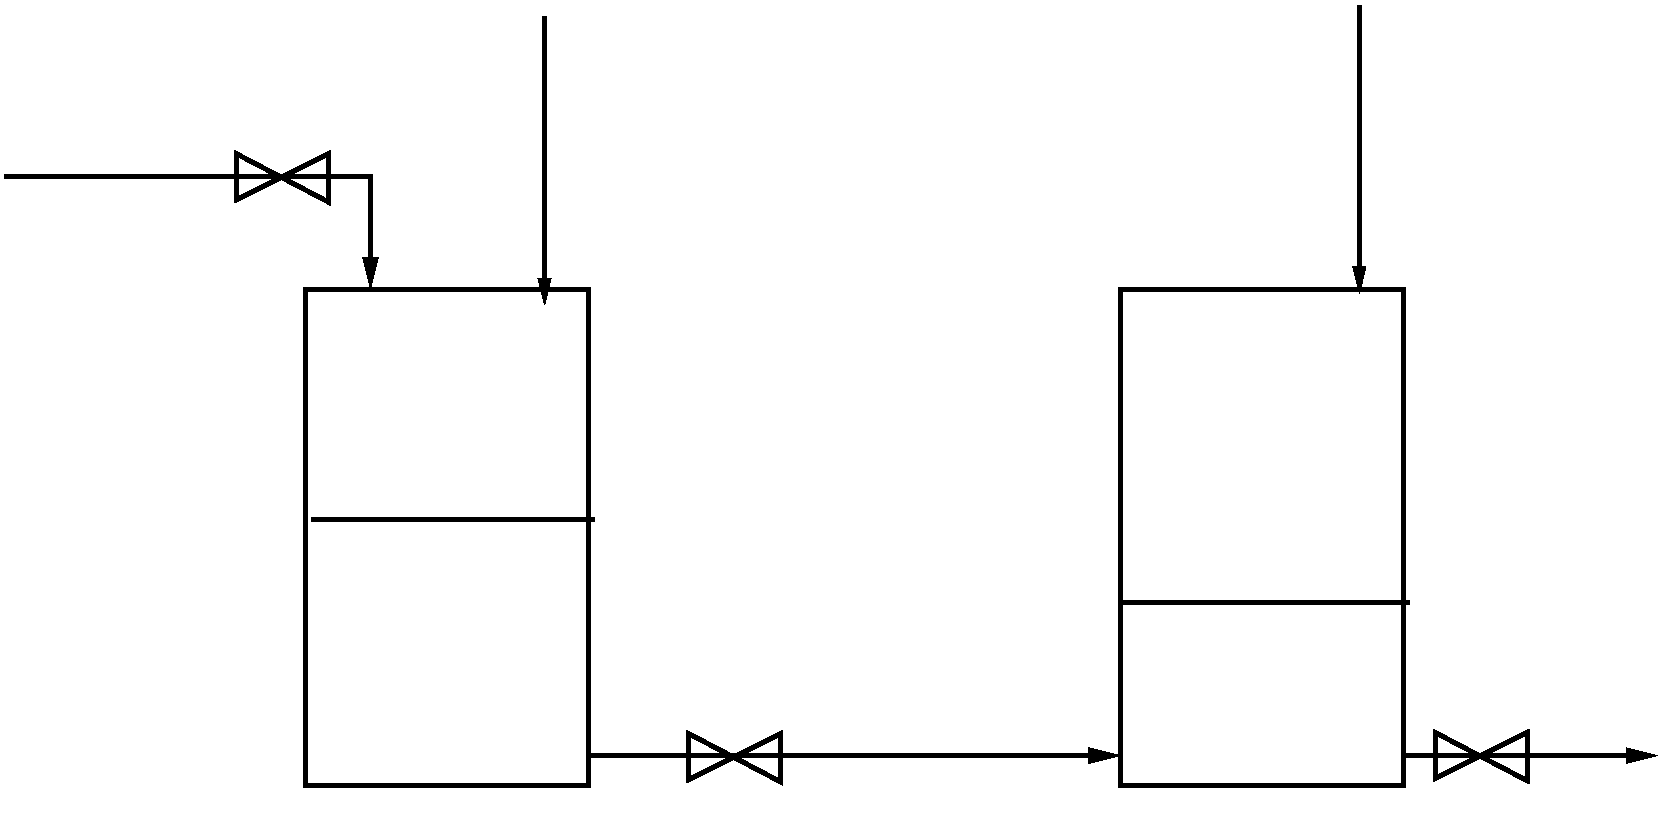
\includegraphics{mpc/two_tanks}%
\end{picture}%
\setlength{\unitlength}{4144sp}%
%
\begingroup\makeatletter\ifx\SetFigFont\undefined%
\gdef\SetFigFont#1#2#3#4#5{%
  \reset@font\fontsize{#1}{#2pt}%
  \fontfamily{#3}\fontseries{#4}\fontshape{#5}%
  \selectfont}%
\fi\endgroup%
\begin{picture}(12666,6356)(688,-5390)
\put(11881,-5326){\makebox(0,0)[lb]{\smash{{\SetFigFont{20}{24.0}{\rmdefault}{\mddefault}{\updefault}{\color[rgb]{0,0,0}$u_{22}$}%
}}}}
\put(1216,-646){\makebox(0,0)[lb]{\smash{{\SetFigFont{20}{24.0}{\rmdefault}{\mddefault}{\updefault}{\color[rgb]{0,0,0}$u_{11}$}%
}}}}
\put(9991,-4471){\makebox(0,0)[lb]{\smash{{\SetFigFont{20}{24.0}{\rmdefault}{\mddefault}{\updefault}{\color[rgb]{0,0,0}$x_2$}%
}}}}
\put(3871,-4021){\makebox(0,0)[lb]{\smash{{\SetFigFont{20}{24.0}{\rmdefault}{\mddefault}{\updefault}{\color[rgb]{0,0,0}$x_1$}%
}}}}
\put(6886,-5101){\makebox(0,0)[lb]{\smash{{\SetFigFont{20}{24.0}{\rmdefault}{\mddefault}{\updefault}{\color[rgb]{0,0,0}$u_{12}$}%
}}}}
\put(5041,-1006){\makebox(0,0)[lb]{\smash{{\SetFigFont{20}{24.0}{\rmdefault}{\mddefault}{\updefault}{\color[rgb]{0,0,0}$w_1$}%
}}}}
\put(11251,-1096){\makebox(0,0)[lb]{\smash{{\SetFigFont{20}{24.0}{\rmdefault}{\mddefault}{\updefault}{\color[rgb]{0,0,0}$w_2$}%
}}}}
\end{picture}%
}
%\caption{Two tank system}
%\label{fig:two_tanks}
%\end{figure*}
%
%We assume that the nominal value of $w_{1,n} = 0.1$ and that of $w_{2,n} =
%5$. The set $\mathbb{W}$ is given by $\mathbb{W} := \set{w \mid 0\leq
%  w_1\leq 0.2, 0 \leq w_2 \leq 10}$.
%
%The input constraints are given by $\mathbb{U}_1 = \set {u_1 \mid 0
%  \leq u_{11} \leq 10, 0 \leq u_{12} \leq 10}$ and $\mathbb{U}_2 =
%\set{u_2 \mid 0 \leq u_{22} \leq 20}$.
%
%Note that since we have a system of integrators, any level in the tank
%can be stabilized as long as all the flows in the system are
%balanced. Therefore, we choose the steady state in the tank as $x_s =
%(20,20)$ (the level in both tanks are 20). The input steady state is
%obtained by solving the following optimization problem
%\[ min_{u}{u'Ru} \qquad \text{s.t~} Bu = -w_n ; u \in \mathbb{U} \]
%in which $w_n$ is the nominal disturbance. For the choice of $R = I$
%($I$ denotes the identity matrix), the input steady-state is obtained
%as $u_s = (3.2667,3.3667,8.3667)$. 
%
%The stage cost was chosen as $\ell(x,u) = 0.1 x'x + u'u$. We solve the
%MPC problem in deviation variables, so that regulation to the origin
%implies regulation to the steady state mentioned above. Following
%the design procedure outlined in the previous sections, we chose 
%(i) $V_f(x) = x'Px,\kappa_f(x) = Kx$ as the solution to the Riccatti
%equation, 
%(ii)$a$ = 1 and the terminal region as $x'Px \leq 1$. The choice of
%  $a=1$ satisfies the requirements in Assumption \ref{ass:bsa}, (iii)
%$\bar{V} = 100$, (iv) a prediction horizon of $N=15$ and (v)the controller that corrects for the error between the nominal
%  and actual states was also chosen as $K(x-z)$ in which $K = \kappa_f(x)$.
%
%For these choice of parameters, we followed the algorithm mentioned in
%\citet{rakovic:kerrigan:kouramas:mayne:2003} to find the set
%$\mathbb{V}$ (we chose $N=200$ and $\alpha = 1e-6$). Note that, since the original input set contained no
%coupled inputs, the tightened set also contains no coupled inputs. 
%
%In Figure \ref{fig:CL1}, we show the closed-loop response 
%nominal closed-loop response of the level in the second tank and the for cooperative MPC rejecting a
%persistent disturbance $w_k \in \mathbb{W}$.  We also show the cost-function $V_N(z,\tilde{\mathbf{v}})$ and
%$V_N(x,\tilde{\mathbf{v}})$ to show that although the warm-start was
%infeasible for the actual state, it was still feasible for the nominal
%state and hence we could obtain the closed-loop guarantees for robust
%cooperative MPC. Note that, for this particular disturbance
%realization, we could not reset the nominal state to the actual state.
%
%\begin{figure*}
%\centering
%\scriptsize
%\resizebox{1\textwidth}{!}{% GNUPLOT: LaTeX picture with Postscript
\begingroup
  \makeatletter
  \providecommand\color[2][]{%
    \GenericError{(gnuplot) \space\space\space\@spaces}{%
      Package color not loaded in conjunction with
      terminal option `colourtext'%
    }{See the gnuplot documentation for explanation.%
    }{Either use 'blacktext' in gnuplot or load the package
      color.sty in LaTeX.}%
    \renewcommand\color[2][]{}%
  }%
  \providecommand\includegraphics[2][]{%
    \GenericError{(gnuplot) \space\space\space\@spaces}{%
      Package graphicx or graphics not loaded%
    }{See the gnuplot documentation for explanation.%
    }{The gnuplot epslatex terminal needs graphicx.sty or graphics.sty.}%
    \renewcommand\includegraphics[2][]{}%
  }%
  \providecommand\rotatebox[2]{#2}%
  \@ifundefined{ifGPcolor}{%
    \newif\ifGPcolor
    \GPcolortrue
  }{}%
  \@ifundefined{ifGPblacktext}{%
    \newif\ifGPblacktext
    \GPblacktexttrue
  }{}%
  % define a \g@addto@macro without @ in the name:
  \let\gplgaddtomacro\g@addto@macro
  % define empty templates for all commands taking text:
  \gdef\gplbacktext{}%
  \gdef\gplfronttext{}%
  \makeatother
  \ifGPblacktext
    % no textcolor at all
    \def\colorrgb#1{}%
    \def\colorgray#1{}%
  \else
    % gray or color?
    \ifGPcolor
      \def\colorrgb#1{\color[rgb]{#1}}%
      \def\colorgray#1{\color[gray]{#1}}%
      \expandafter\def\csname LTw\endcsname{\color{white}}%
      \expandafter\def\csname LTb\endcsname{\color{black}}%
      \expandafter\def\csname LTa\endcsname{\color{black}}%
      \expandafter\def\csname LT0\endcsname{\color[rgb]{1,0,0}}%
      \expandafter\def\csname LT1\endcsname{\color[rgb]{0,1,0}}%
      \expandafter\def\csname LT2\endcsname{\color[rgb]{0,0,1}}%
      \expandafter\def\csname LT3\endcsname{\color[rgb]{1,0,1}}%
      \expandafter\def\csname LT4\endcsname{\color[rgb]{0,1,1}}%
      \expandafter\def\csname LT5\endcsname{\color[rgb]{1,1,0}}%
      \expandafter\def\csname LT6\endcsname{\color[rgb]{0,0,0}}%
      \expandafter\def\csname LT7\endcsname{\color[rgb]{1,0.3,0}}%
      \expandafter\def\csname LT8\endcsname{\color[rgb]{0.5,0.5,0.5}}%
    \else
      % gray
      \def\colorrgb#1{\color{black}}%
      \def\colorgray#1{\color[gray]{#1}}%
      \expandafter\def\csname LTw\endcsname{\color{white}}%
      \expandafter\def\csname LTb\endcsname{\color{black}}%
      \expandafter\def\csname LTa\endcsname{\color{black}}%
      \expandafter\def\csname LT0\endcsname{\color{black}}%
      \expandafter\def\csname LT1\endcsname{\color{black}}%
      \expandafter\def\csname LT2\endcsname{\color{black}}%
      \expandafter\def\csname LT3\endcsname{\color{black}}%
      \expandafter\def\csname LT4\endcsname{\color{black}}%
      \expandafter\def\csname LT5\endcsname{\color{black}}%
      \expandafter\def\csname LT6\endcsname{\color{black}}%
      \expandafter\def\csname LT7\endcsname{\color{black}}%
      \expandafter\def\csname LT8\endcsname{\color{black}}%
    \fi
  \fi
  \setlength{\unitlength}{0.0500bp}%
  \begin{picture}(7200.00,3024.00)%
    \gplgaddtomacro\gplbacktext{%
      \csname LTb\endcsname%
      \put(814,704){\makebox(0,0)[r]{\strut{} 0}}%
      \put(814,1218){\makebox(0,0)[r]{\strut{} 10}}%
      \put(814,1732){\makebox(0,0)[r]{\strut{} 20}}%
      \put(814,2245){\makebox(0,0)[r]{\strut{} 30}}%
      \put(814,2759){\makebox(0,0)[r]{\strut{} 40}}%
      \put(946,484){\makebox(0,0){\strut{} 0}}%
      \put(1433,484){\makebox(0,0){\strut{} 10}}%
      \put(1921,484){\makebox(0,0){\strut{} 20}}%
      \put(2408,484){\makebox(0,0){\strut{} 30}}%
      \put(2896,484){\makebox(0,0){\strut{} 40}}%
      \put(3383,484){\makebox(0,0){\strut{} 50}}%
      \put(176,1731){\rotatebox{-270}{\makebox(0,0){\strut{}Level in Tank-2}}}%
      \put(2164,154){\makebox(0,0){\strut{}Time}}%
      \put(2165,1115){\makebox(0,0)[l]{\strut{}$S_K(\infty)$ bound}}%
    }%
    \gplgaddtomacro\gplfronttext{%
      \csname LTb\endcsname%
      \put(2396,2586){\makebox(0,0)[r]{\strut{}Actual}}%
      \csname LTb\endcsname%
      \put(2396,2366){\makebox(0,0)[r]{\strut{}Nominal}}%
    }%
    \gplgaddtomacro\gplbacktext{%
      \csname LTb\endcsname%
      \put(4109,484){\makebox(0,0){\strut{} 0}}%
      \put(4517,484){\makebox(0,0){\strut{} 2}}%
      \put(4925,484){\makebox(0,0){\strut{} 4}}%
      \put(5334,484){\makebox(0,0){\strut{} 6}}%
      \put(5742,484){\makebox(0,0){\strut{} 8}}%
      \put(6150,484){\makebox(0,0){\strut{} 10}}%
      \put(6282,704){\makebox(0,0)[l]{\strut{} 0}}%
      \put(6282,1115){\makebox(0,0)[l]{\strut{} 100}}%
      \put(6282,1526){\makebox(0,0)[l]{\strut{} 200}}%
      \put(6282,1937){\makebox(0,0)[l]{\strut{} 300}}%
      \put(6282,2348){\makebox(0,0)[l]{\strut{} 400}}%
      \put(6282,2759){\makebox(0,0)[l]{\strut{} 500}}%
      \put(7051,1731){\rotatebox{-270}{\makebox(0,0){\strut{}Cost}}}%
      \put(5129,154){\makebox(0,0){\strut{}time}}%
    }%
    \gplgaddtomacro\gplfronttext{%
      \csname LTb\endcsname%
      \put(5163,2586){\makebox(0,0)[r]{\strut{}$V_N^\beta(x,\tilde{\mathbf{v}})$}}%
      \csname LTb\endcsname%
      \put(5163,2366){\makebox(0,0)[r]{\strut{}$V_N^\beta(z,\tilde{\mathbf{v}})$}}%
      \csname LTb\endcsname%
      \put(5163,2146){\makebox(0,0)[r]{\strut{}$\bar{V}$}}%
    }%
    \gplbacktext
    \put(0,0){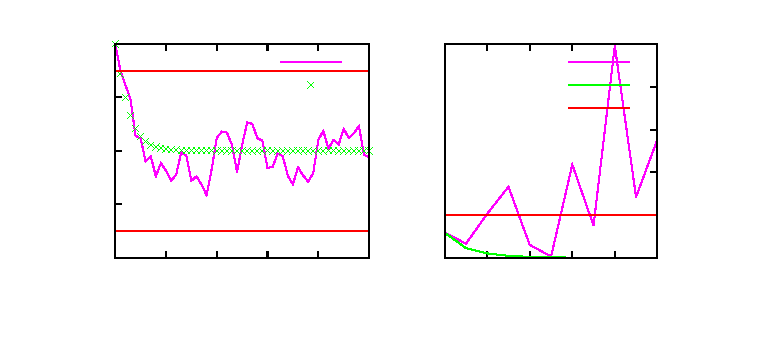
\includegraphics{mpc/CL1}}%
    \gplfronttext
  \end{picture}%
\endgroup
}
%\caption{(Left) Closed-loop response (Right) Warm start rendered
%  infeasible for actual state because of disturbance}
%\label{fig:CL1}
%\end{figure*}
%
%
%In Figure \ref{fig:CL2}, we show the closed-loop response using a
%modified version of Algorithm \ref{alg:rcoop}. The modification we
%made are to reset the nominal state to the actual state at time $k$ if the
%following conditions are satisfied (i)The nominal state $z(k)$ is inside $\mathbb{Z}_f$.
%(ii) The warm start $\tilde{\mathbf{v}}(k)$ is feasible for the
%actual state $x(k)$ and , (iii) The time elapsed since the last reset
%is greater than $\bar{T}$
%time periods (we chose $\bar{T} = 10$)
%
%\begin{figure*}
%\centering
%\scriptsize
%\resizebox{1\textwidth}{!}{% GNUPLOT: LaTeX picture with Postscript
\begingroup
  \makeatletter
  \providecommand\color[2][]{%
    \GenericError{(gnuplot) \space\space\space\@spaces}{%
      Package color not loaded in conjunction with
      terminal option `colourtext'%
    }{See the gnuplot documentation for explanation.%
    }{Either use 'blacktext' in gnuplot or load the package
      color.sty in LaTeX.}%
    \renewcommand\color[2][]{}%
  }%
  \providecommand\includegraphics[2][]{%
    \GenericError{(gnuplot) \space\space\space\@spaces}{%
      Package graphicx or graphics not loaded%
    }{See the gnuplot documentation for explanation.%
    }{The gnuplot epslatex terminal needs graphicx.sty or graphics.sty.}%
    \renewcommand\includegraphics[2][]{}%
  }%
  \providecommand\rotatebox[2]{#2}%
  \@ifundefined{ifGPcolor}{%
    \newif\ifGPcolor
    \GPcolortrue
  }{}%
  \@ifundefined{ifGPblacktext}{%
    \newif\ifGPblacktext
    \GPblacktexttrue
  }{}%
  % define a \g@addto@macro without @ in the name:
  \let\gplgaddtomacro\g@addto@macro
  % define empty templates for all commands taking text:
  \gdef\gplbacktext{}%
  \gdef\gplfronttext{}%
  \makeatother
  \ifGPblacktext
    % no textcolor at all
    \def\colorrgb#1{}%
    \def\colorgray#1{}%
  \else
    % gray or color?
    \ifGPcolor
      \def\colorrgb#1{\color[rgb]{#1}}%
      \def\colorgray#1{\color[gray]{#1}}%
      \expandafter\def\csname LTw\endcsname{\color{white}}%
      \expandafter\def\csname LTb\endcsname{\color{black}}%
      \expandafter\def\csname LTa\endcsname{\color{black}}%
      \expandafter\def\csname LT0\endcsname{\color[rgb]{1,0,0}}%
      \expandafter\def\csname LT1\endcsname{\color[rgb]{0,1,0}}%
      \expandafter\def\csname LT2\endcsname{\color[rgb]{0,0,1}}%
      \expandafter\def\csname LT3\endcsname{\color[rgb]{1,0,1}}%
      \expandafter\def\csname LT4\endcsname{\color[rgb]{0,1,1}}%
      \expandafter\def\csname LT5\endcsname{\color[rgb]{1,1,0}}%
      \expandafter\def\csname LT6\endcsname{\color[rgb]{0,0,0}}%
      \expandafter\def\csname LT7\endcsname{\color[rgb]{1,0.3,0}}%
      \expandafter\def\csname LT8\endcsname{\color[rgb]{0.5,0.5,0.5}}%
    \else
      % gray
      \def\colorrgb#1{\color{black}}%
      \def\colorgray#1{\color[gray]{#1}}%
      \expandafter\def\csname LTw\endcsname{\color{white}}%
      \expandafter\def\csname LTb\endcsname{\color{black}}%
      \expandafter\def\csname LTa\endcsname{\color{black}}%
      \expandafter\def\csname LT0\endcsname{\color{black}}%
      \expandafter\def\csname LT1\endcsname{\color{black}}%
      \expandafter\def\csname LT2\endcsname{\color{black}}%
      \expandafter\def\csname LT3\endcsname{\color{black}}%
      \expandafter\def\csname LT4\endcsname{\color{black}}%
      \expandafter\def\csname LT5\endcsname{\color{black}}%
      \expandafter\def\csname LT6\endcsname{\color{black}}%
      \expandafter\def\csname LT7\endcsname{\color{black}}%
      \expandafter\def\csname LT8\endcsname{\color{black}}%
    \fi
  \fi
  \setlength{\unitlength}{0.0500bp}%
  \begin{picture}(7200.00,3024.00)%
    \gplgaddtomacro\gplbacktext{%
      \csname LTb\endcsname%
      \put(814,704){\makebox(0,0)[r]{\strut{} 10}}%
      \put(814,1389){\makebox(0,0)[r]{\strut{} 20}}%
      \put(814,2074){\makebox(0,0)[r]{\strut{} 30}}%
      \put(814,2759){\makebox(0,0)[r]{\strut{} 40}}%
      \put(946,484){\makebox(0,0){\strut{} 0}}%
      \put(2898,484){\makebox(0,0){\strut{} 10}}%
      \put(4851,484){\makebox(0,0){\strut{} 20}}%
      \put(6803,484){\makebox(0,0){\strut{} 30}}%
      \put(176,1731){\rotatebox{-270}{\makebox(0,0){\strut{}Inventory at Retailer}}}%
      \put(3874,154){\makebox(0,0){\strut{}Time}}%
      \put(4851,1732){\makebox(0,0)[l]{\strut{}Nominal state reset}}%
    }%
    \gplgaddtomacro\gplfronttext{%
      \csname LTb\endcsname%
      \put(4037,877){\makebox(0,0)[r]{\strut{}Actual}}%
      \csname LTb\endcsname%
      \put(5816,877){\makebox(0,0)[r]{\strut{}Nominal}}%
    }%
    \gplbacktext
    \put(0,0){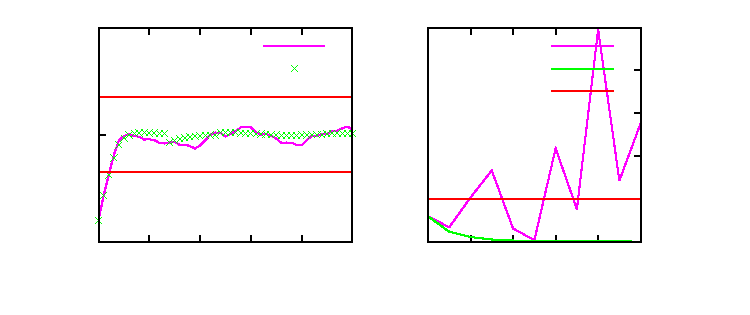
\includegraphics{CL2}}%
    \gplfronttext
  \end{picture}%
\endgroup
}
%\caption{(Left) Closed-loop response. Notice that we reset the state
%  around t = 15 (Right) Warm start rendered
%  infeasible for actual state because of disturbance}
%\label{fig:CL2}
%\end{figure*}
%


\section{Related Work}
\label{sec:related}
Cooperative MPC has evolved as a attractive architecture for
distributed control because it solves the centralized control
problem, and inherits the desirable closed-loop properties of
centralized control. 
In Cooperative MPC, the centralized optimization
problem is solved directly using parallel optimization
architectures. \citet{liu:chen:pena:christofides:2010}  use an algorithm similar to cooperative MPC to solve the centralized control problem for non-linear systems. They obtain the warm start by using a closed form controller $\bu = h(x)$ that satisfies all the criteria in the Lyapunov theorem to establish asymptotic stability. This controller is called the reference controller and the online controller is designed to improve the performance of  the reference control. The authors propose algorithms based on the  Jacobi algorithm (all subsystems optimize in parallel) and the Gauss-Seidel algorithm (subsystems optimize in sequence). The stability theorem is based on suboptimal MPC. However, since the centralized problem has coupled constraints, their algorithm does not provide performance guarantee. Cooperative MPC based on relaxing the terminal region has been proposed for non-linear systems by \citet{stewart:wright:rawlings:2011}. The parallel optimization algorithm is an modification of the Jacobi algorithm. The modification is based on a sequential evaluation of objective functions to obtain a descent direction (without requiring a coordinator).

As mentioned earlier, an important requirement for cooperative MPC is that the subsystems share objective functions and models with each other. For situations in which it is not feasible for the subsystem to share objectives and models, 
 \citet{maestre:pena:camacho:alamo:2011} propose a distributed MPC algorithm  based on agent negotiation. In this algorithm, each subsystem solves its local optimization problem, but on the entire input sequence (including the inputs from other subsystems). In the second phase of the algorithms, the subsystems share their proposed solution with other subsystems. Finally, each subsystem calculates the objective value and constraint violation of the solutions from every other subsystem and broadcasts them. The subsystems then negotiate to obtain a feasible input sequence. By using warm start and algorithm design to accept only input sequences that decrease the cost, the algorithm establishes closed-loop properties by using suboptimal MPC. 
The drawback of the proposed architecture is 
that  the agents have to solve larger optimization problems
(because they have to optimize over all the inputs that affect their state).

 \citet{maestre:pena:camacho:2011}  use a game theory based distributed optimization algorithm to implement distributed MPC. Similar to \citet{maestre:pena:camacho:alamo:2011}, the subsystems do not share models or objectives. In this algorithm, each subsystem broadcasts their current iterate to all the other subsystems. Upon receiving the iterates, the subsystems optimize for their input decisions keeping the other inputs fixed. Next, these optimized inputs are broadcast to the other subsystems. Next, each subsystem evaluates all possible combinations of previous iterate and current optimal solutions to come up with a list of (centralized input, local objective) pair that is broadcast. Each subsystem can now sum over the local objectives to find the centralized input with best cost-drop. While, stability is guaranteed by design of warm start and design of the terminal region, there are no convergence guarantees of the algorithm.

 \citet{muller:revle:allgower:2012} decouple the terminal region constraint by providing a method that finds time varying local terminal regions that when satisfied by each subsystem, also satisfies the centralized terminal region. In their algorithm, the authors assume that subsystems do not share models and objectives. Hence, after performing local optimizations, input directions that do not reduce cost or input directions that are infeasible are discarded. Stability is established by using suboptimal MPC theory. 
 
 In the methods mentioned above, the parallel optimization algorithm has been designed to minimize a centralized cost when the subsystems do not know the centralized cost and/or constraints. These optimization algorithms are also designed satisfy the requirements of suboptimal MPC (feasible iterates, cost-drop at each iterate). However, the convergence properties and performance guarantees from these algorithms have not be studied.
 
Problems like multi-vehicle synchronization have a unique feature, in that, the dynamics of the different subsystems are uncoupled ($x_i$ depends only on $u_i$). In such problems, the objective function is separable, and the only complicating constraint is the consensus point (which is similar to terminal equality constraint). In \citet{johansson:speranzon:johansson:johansson:2006}, a primal decomposition is used to solve such control problems. The algorithm uses a coordinator to resolve the coupled constraint.

The distributed MPC algorithms mentioned above focus on designing a parallel optimization algorithm that satisfies the requirements of suboptimal MPC. As mentioned earlier, another family of methods for distributed MPC focus on solving the centralized optimization problem using a parallel optimization algorithm efficiently, and utilizing optimal MPC stability theory to provide guaranteed close-loop properties. These methods, typically focus on optimizing the dual of the online optimization problem using parallel solvers (with each solver representing a subsystem). The algorithms based on the dual decomposition converge to the centralized optimal solution for convex optimization problem with coupled constraints . The main disadvantage of these parallel optimization algorithms are that they (i) employ a coordinator that updates the Lagrange multiplier based on the subsystem solutions and, (ii) provide no guarantees on the feasibility of intermediate iterates. The second inequality implies that we have to wait till convergence before obtaining a feasible input.

There are many distributed algorithms using dual decomposition based on different parallel optimization algorithms used.

Subgradient methods are  used in \citet{cheng:forbes:yip:2007},\citet{ma:anderson:borrelli:2011},
\citet{wakasa:arakawa:tanka:akashi:2008},
\citet{marcos:forbes:guay:2009}. 

\citet{morocan:bourdais:dumur:buisson:2011} use Benders decomposition to solve a building control problem.

\citet{scheu:marquardt:2011}  augment the
local subsystem objective function with the sensitivity of the
objectives and constraints of other subsystems to obtain updates for
the dual variables along with the primal variables. Thus, their algorithm does not require a coordinating layer.However, this
method generates a feasible solution only upon
convergence.

 \citet{giselsson:doan:keviczky:schutter:rantzer:2012}, \citet{giselsson:rantzer:2010}
propose a dual decomposition algorithm with a stopping criteria based
on the objective value to ensure stability. They advocate the use of
long prediction horizon along with results obtained in
\citet{grune:2009} to determine bounds on the value of the objective
function so that stability can be guaranteed.

 \citet{doan:keviczky:necoara:diehl:schutter:2009} modified
the Han's algorithm which is a dual decomposition based algorithm for
the special structure of the MPC problem. Although the method uses
communication between directly connected subsystems, stability is
guaranteed only upon convergence. \citet{necoara:doan:suykens:2008}
use a smoothing technique to simplify the dual problem. With the
smoothing technique, the coordinator problem for finding the Lagrange
multiplier updates becomes easier. The algorithm also gives bounds on
the number of iterations so that the optimal solution and constraint
violation are within a pre-specified limit ($\epsilon$ approximation of
the centralized problem). The main advantage is that the dual
decomposition based on proximal center is order of magnitude faster
than other sub-gradient based methods. Finally,
\citet{doan:keviczky:schutter:2011}, propose a primal feasible dual
gradient approach, that generates a primal feasible solution  that
achieves cost-drop in a
finite number of iterations based on an averaging scheme of the primal
variables at each iteration. 

\citet{christofides:scattolini:pena:liu:2012} is a recent review of different algorithms for distributed
MPC. \citet{necoara:nedelcu:dumitrache:2011} provides an excellent overview of the different
optimization problems and parallel solution strategies that are seen
in control and estimation.

\citet{trodden:richards:2006,trodden:richards:2007} propose a tube based robust distributed
MPC algorithm. In their method, at each sampling time, only one
subsystem performs optimization. The subsystem optimizes only over its
decision variables, keeping all other subsystem decisions fixed from
the previous iteration.. \citet{richards:how:2004} present a robust tube-based
MPC for systems with decoupled dynamics. The coupling constraints are
coupled output constraints. Their algorithm is based on the
Gauss-Siedel iterations.



\section{Conclusions}
\label{sec:conclusions}
We propose a cooperative MPC algorithm in which each agent solves the
centralized optimization problem subject to its own inputs. The
algorithm uses a primal decomposition to solve the centralized problem
using a Jacobi algorithm. Stability is ensured by designing
appropriate terminal region and penalties and using suboptimal MPC theory.
The advantages of using the cooperative MPC algorithm are (i) Guaranteed closed-loop properties, (ii) The optimization problems solved by the subsystems are of the same complexity if they subsystems were just optimizing its local control problem (in terms of the size of the optimization problem), (iii) No coordinators are required and (iv) There are no requirements on number of iterations to be made. In fact. the cooperative MPC is truly parallel in the sense that one or more subsystems can go offline and we can still find feasible inputs. 
The drawbacks of the cooperative MPC algorithm are that (i) Each subsystem has to share objective and constraints and (ii) Performance guarantee, that of converging to the centralized optimal solution, can only be guaranteed to a special class of problems that have uncoupled constraints. We believe that for many applications, sharing objectives and constraints would not be a bottleneck. For example, coordinating controllers inside a single plant. For the second drawback, we review two relaxations of the centralized online control problem so that the relaxations do not have coupled constraints. While the first relaxation based on sub-states is not applicable to all systems, the second relaxation based on magnifying the terminal penalty is applicable to all systems. The relaxations, however, add restrictions on the feasible set over which the centralized problem is defined. That is, compared to the centralized control problem, the relaxed centralized control problems have smaller region of attraction. Finally, we used techniques from MPC using tubes to propose
a robust cooperative MPC controller that has both stability and
performance guarantees.
\bibliographystyle{abbrvnat}
{\bibliography{abbreviations,articles,proceedings,books,unpub}
}
\end{document}











